\section{Introduction and Problem Formulation}
\label{sec:intro}

Magnetic Resonance Imaging (MRI) is a cornerstone of non-invasive medical diagnostics, yet its inherently slow acquisition time remains a critical bottleneck. Accelerating MRI typically involves undersampling the $k$-space and solving a highly ill-posed inverse problem \citep{chung2022score}. While deep generative models have achieved remarkable success in MRI reconstruction, the vast majority of these approaches operate strictly on magnitude images in the spatial domain, entirely discarding the complex phase information.

This magnitude-only paradigm creates a research gap, as emerging complex-valued networks demonstrate superior signal fidelity in raw MRI processing \citep{rempe2026kvit, dou2025mri}. However, the lack of realistic, fully complex synthetic data severely limits data augmentation and the robust validation of complex-valued reconstruction algorithms. While recent diffusion approaches \citep{rempe2025phasegen} explore complex-valued generation, their lack of explicit phase topology preservation leaves a critical need for geometrically grounded baselines. Naive generative models operating without complex-domain geometric constraints are prone to hallucinating non-physical phase discontinuities, which upon Forward Fast Fourier Transform (FFT) leak into measured $k$-space subspaces and corrupt high-frequency anatomical details.

Current approaches suffer from a fundamental topological mismatch: they naively treat the complex signal as a flat, two-channel tensor embedded in a Euclidean space $\mathbb{C} \cong \mathbb{R}^2$ \citep{chung2022score}. This ignores the intrinsic circular topology ($S^1$) of the signal's phase. Consequently, standard Euclidean interpolation suffers from destructive interference due to the triangle inequality, $|z(t)| = |(1-t)z_0 + t z_1| \le (1-t)|z_0| + t|z_1|$, with strict inequality whenever phases differ ($\theta_0 \ne \theta_1$). Under an independent uniform phase prior $\theta_0 \sim \mathcal{U}(S^1)$, the expected mid-point ($t=0.5$) magnitude attenuation is analytically $1 - \mathbb{E}|\cos(\Delta\theta/2)| = 1 - 2/\pi \approx 36.3\%$ (empirically $\sim$16\% on spatially correlated MRI data). Furthermore, flat angular interpolation does not respect wrapping at the boundary ($-\pi \sim \pi$). These effects motivate evaluating a geometry-aware probability path for complex MRI data.

To bridge the gap between generative modeling and the structured nature of physical signals, we propose \textbf{Cylindrical Flow Matching}, a geometry-aware generative framework designed specifically for complex-valued medical image synthesis. Building on flow matching \citep{lipman2023flow} and its manifold extension \citep{chen2024flow}, we hypothesize that radial-angular paths provide a better inductive bias than Cartesian coordinates, natively resolving phase discontinuities.

In summary, our contributions are as follows:
\begin{itemize}
    \item We define the representation, geometry, loss, and inference procedure for \textbf{Cylindrical Flow Matching}, modeling nonnegative physical amplitudes on $\mathbb{R}_+$ and numerical phase coordinates on $S^1$.
    \item We test this hypothesis through controlled ablations on complex-valued generation against a standard Euclidean baseline, demonstrating that substituting the Euclidean assumption natively prevents phase discontinuities and signal cancellation.
    \item We demonstrate the practical value of this geometry-aware prior in a downstream reconstruction experiment using simulated Cartesian $k$-space undersampling.
\end{itemize}

% ----------------------------------------
\begin{figure}[t]
    \centering
    \begin{subfigure}[b]{0.48\textwidth}
        \centering
        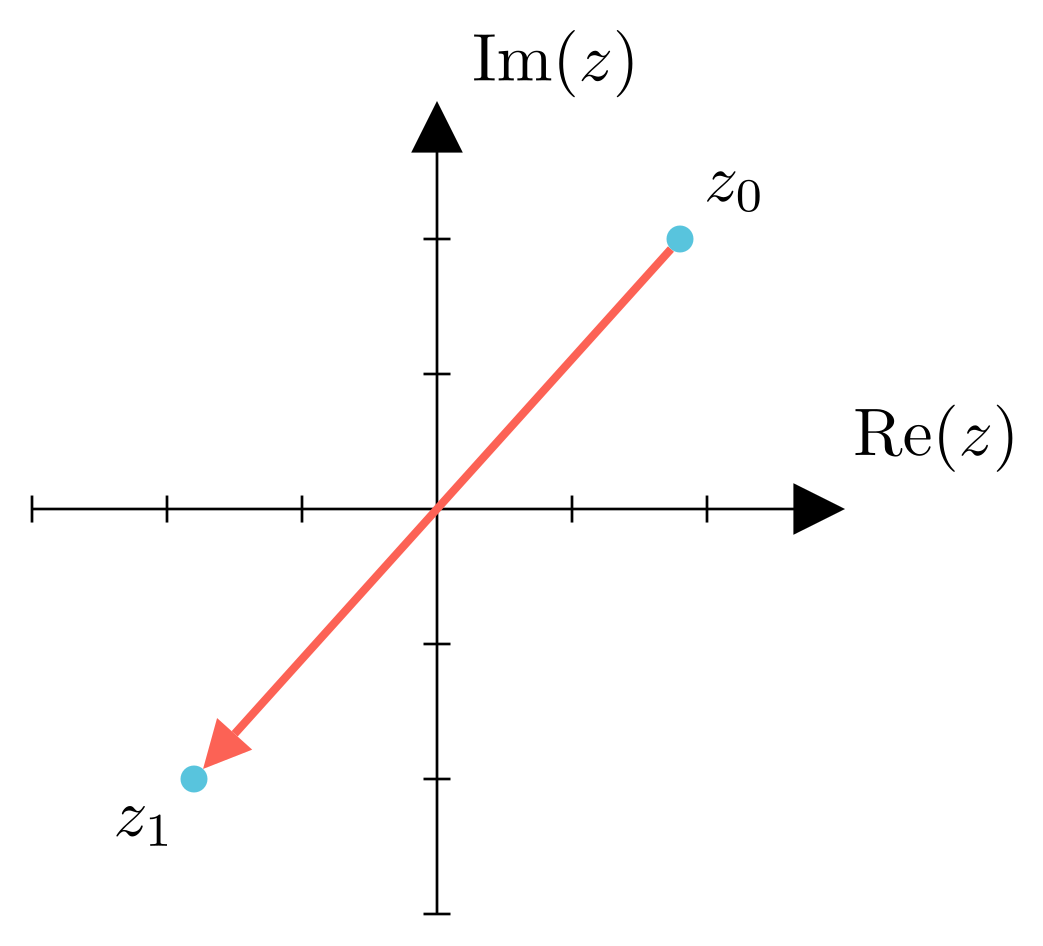
\includegraphics[height=4.0cm, keepaspectratio]{figures/EuclideanFlow_cropped.png}
        \caption{Standard Euclidean Flow ($\mathbb{R}^2$)}
        \label{fig:flow_euclidean}
    \end{subfigure}
    \hfill
    \begin{subfigure}[b]{0.48\textwidth}
        \centering
        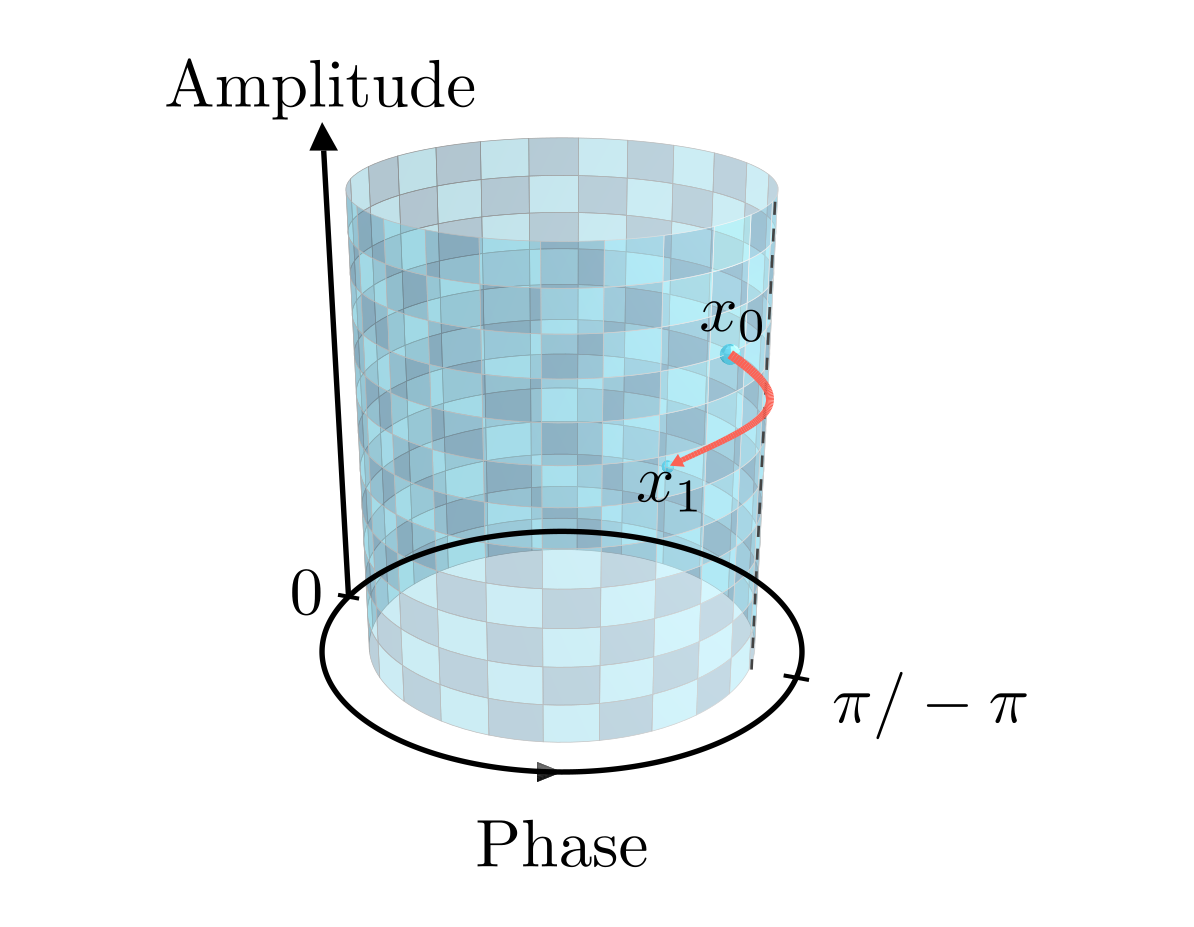
\includegraphics[height=4.0cm, keepaspectratio]{figures/CylindricalFlow_cropped.png}
        \caption{Cylindrical Flow Matching (Ours)}
        \label{fig:flow_cylindrical}
    \end{subfigure}
    \caption{\textbf{Topological mismatch in complex-valued generation.} \textbf{(a)} In the complex plane $(\mathrm{Re}(z), \mathrm{Im}(z))$, linear interpolation between antipodal states $z_0$ and $z_1$ passes through the origin, causing amplitude attenuation ($|z_{1/2}| \ll \frac{1}{2}(|z_0| + |z_1|)$). \textbf{(b)} Cylindrical Flow Matching follows the shortest angular path on $S^1$ while interpolating amplitude separately.}
    \label{fig:teaser_flow}
    \vspace{-2mm}
\end{figure}
% ----------------------------------------
